\section{Goals}

The main goal of using \textit{Linux Security Modules} in combination with WebAssembly
is to provide a finer grain customisation when choosing how to limit the permissions given
to the executable. More specifically, the desired features are:
\begin{enumerate}
  \item to give the possibility to differentiate between directories and files when giving permissions;
  \item to clearly separate different capabilities;
  \item to extend the possible set of permissions under the user's control.
\end{enumerate}

Additional desirable features include the possibility to apply exceptions to a certain rule, as well
as limiting the access to other resources in the operating systems, such as network, devices, and
inter-process communications.

Finally, usability is also taken into consideration, especially an user's point of view.

Note that the main purpose of these tests is not to replicate all the functionalities given by
the WebAssembly runtimes (\textit{Wasmtime} and \textit{Wasmer}), but to see how their basic features,
especially running a WebAssembly compiled binary through WASI, can be integrated and/or extended with
security tools from the Linux kernel.
This means that, for example, running a single function exported from a WebAssembly module won't be taken
into consideration.

\section{Restricting the WASI sandbox with Landlock}
\label{sec:restricting-wasi-landlock}

For the integration with Landlock, a new project was developed, in order to provide
a custom command line interface that allowed the user to specify with more precision what
the WebAssembly binary is permitted to do on certain folders and files.

The project is open source and the code is available at \url{https://github.com/micheleberetta98/rust-wasm-landlock}.
In order for the project to compile, the Landlock LSM must be enabled in the Linux kernel.

\subsection{Code architecture and description}\label{sec:landlock-code-architecture}

The code itself is written in \textit{Rust}, and makes use of the
\textit{rust-landlock} \cite{rust-landlock} crate
to communicate with Landlock and the \textit{wasmtime} and \textit{wasmtime-wasi} official
crates in order to have a runtime environment to execute a WebAssembly binary.

The project is divided into five modules, which are the following:
\begin{enumerate}
  \item \texttt{args}, used to define and parse the command line arguments that specify the WebAssembly binary,
        the directories to preopen, and the allowed privileges on individual folders and/or files;
  \item \texttt{landlock}, which handles the creation and update of the permissions' ruleset;
  \item \texttt{main}, the module that interfaces with the user;
  \item \texttt{path\_access}, containing a helper structure to track permission for a single path;
  \item and finally \texttt{wasm}, that communicates with the \textit{wasmtime-wasi} and the \textit{wasmtime} crates
        in order to run the provided binaries, as well as preopening directories.
\end{enumerate}

\begin{figure}[ht]
  \centering
  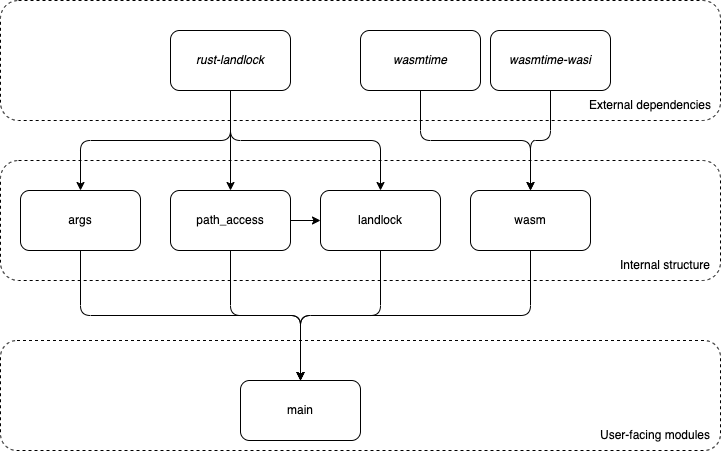
\includegraphics[width=0.8\linewidth]{rust-landlock-code-diagram.png}
  \caption{The code's architecture.}
  \label{fig:rust-landlock-code-architecture}
\end{figure}

\begin{code}[language=rust, caption=The \texttt{Args} struct., label=lst:arg-struct]
pub struct Args {
  // The module to execute
  pub wasm_module: String,

  // The preopened dir(s) to pass to wasmtime
  pub dirs: Vec<String>,

  // The preopened mapped dir(s) to pass to wasmtime
  pub mapdirs: Vec<(String, String)>,

  // A list of the allowed privileges on a
  // particular folder/file
  pub fs_allows: Vec<(String, BitFlags<AccessFs>)>,

  // Disable landlock (test only)
  pub no_landlock: bool,
}
\end{code}

\clearpage
The architecture diagram is shown in Figure \ref{fig:rust-landlock-code-architecture}, where
are outlined the most important external crates and all dependencies between the modules, represented
by directed arrows.

\subsubsection{The \texttt{args} module}
\label{sec:landlock-args-module}

The main definition of this module is the \texttt{Args} struct, visible in Listing \ref{lst:arg-struct},
used to represent the command line interface that allows to specify which permissions to enable
for one or more specific paths.

Every single field is mapped to one command line argument thanks to the \textit{clap} crates which handles the
creation and parsing of the CLI arguments structure.
Their usage and meaning is described in Table \ref{table:landlock-cli-args}.

\begin{table}
  \centering
  \begin{tabular}{|l|l|l|l|}
    \hline
    \textit{Argument} & \textit{Required} & \textit{Description} \\
    \hline\hline
    \textit{WASM module} & Yes & The path to the WASM binary to run \\ \hline
    \texttt{dir} & No & All the directories to preopen \\ \hline
    \texttt{mapdir} & No & Eventual mappings between the directories \\ \hline
    \texttt{fs-allow} & No & All the permitted actions on a single path \\ \hline
    \texttt{no-landlock} & No & Used to disable the self restriction done by landlock \\
    \hline
  \end{tabular}
  \caption{All the available command line arguments.}
  \label{table:landlock-cli-args}
\end{table}

The first argument is positional, and is the path where the WebAssembly module is located.

The \texttt{dir} and \texttt{mapdir} arguments can appear multiple times and are used to list the directories to preopen
so that the WebAssembly module can access them and their contents.
When mapping a directory, in a way similar to the one provided by the \textit{Wasmtime} command line tool, one can make a
directory appear as ``having a different path'' when accessed by the WebAssembly module.

The \texttt{fs-allow} argument is made up of two parts, separated by a colon - a path to apply the restrictions to,
and a series of enabled permissions on that specific path, separated by a comma.
Each permission is mapped one-to-one to the flags provided by Landlock in a manner listed in Table \ref{table:landlock-flags}.
Moreover, there are three useful ``shortcuts'' used to represent common situations - \texttt{$\sim$read}, \texttt{$\sim$write} and \texttt{*}.

A full example of how these arguments work is shown in Figure \ref{fig:args-example}.

Lastly, the \texttt{no-landlock} argument is only for testing purposes - it is off by default, so that
landlock is enabled and self restriction is applied if not explicitly disabled.

\begin{figure}[ht]
  \centering
  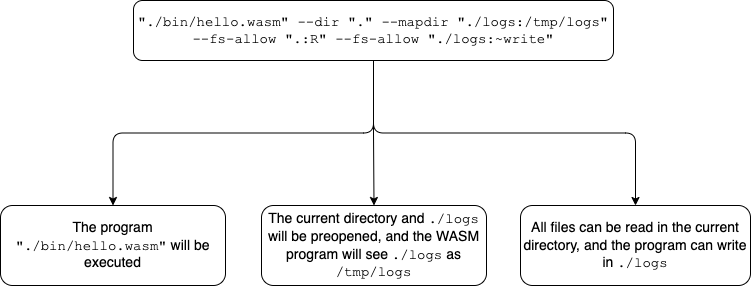
\includegraphics[width=\linewidth]{rust-landlock-args-example.png}
  \caption{A full example of how the arguments are seen by the program.}
  \label{fig:args-example}
\end{figure}

\subsubsection{The \texttt{wasm} module}
\label{sec:landlock-wasm-module}

This module manages a single WebAssembly binary module and forms a bridge to the \textit{wasmtime} and the \textit{wasmtime-wasi}
crates. In this project, \textit{Wasmtime} bindings are used instead of the \textit{Wasmer} ones, but both provide the
same level of functionality, albeit with a different interface. A high level view of the usual sequence in which the steps would be done
when loading and running a module is shown in Figure \ref{fig:wasm-module}, while an outline of the module is visible
in Listing \ref{lst:wasm-module-outline}.

The \textit{WasmModule} structure represents a WASM binary as a vector of bytes, and it also handles the creation
and construction of a \textit{WASI Context}, another structure defined by the \textit{wasmtime-wasi} crate used to store
all preopened directories, eventual imports, and more data that will be useful to run the WebAssembly module.

Moreover, this module defines various helpers to preopen directories, both unmapped and mapped, and
how to run a WebAssembly binary - it must create both an \textit{engine} and a \textit{linker},
as well as a \textit{store}, which represents the memory of a WebAssembly module described in the previous chapter.

Note that the WebAssembly module must have a \textit{default exported function} to run - when compiling with a WASI target,
this is usually represented by the \texttt{\_start} function, which corresponds to the \texttt{main} function in languages
such as C and Rust.

\vspace*{0.5cm}

\begin{code}[language=Rust, caption=The outline of the \texttt{wasm} module., label=lst:wasm-module-outline]
pub struct WasmModule {
  bytes: Vec<u8>, ctx_builder: WasiCtxBuilder,
}

impl WasmModule {
  // Reads the WASM module, initialises WasiCtxBuilder
  pub fn new(path: &str) -> Result<Self> {...}

  // Make the WASM module inherit stdio
  pub fn use_stdio(mut self) -> Self {...}

  // Preopen all given directories
  pub fn preopen_all(
    mut self,
    dirs: &Vec<String>) -> Result<Self> {...}
  
  // Preopen and map all given directories
  pub fn preopen_all_map(
    mut self,
    mapdirs: &Vec<(String, String)>) -> Result<Self> {...}

  // Preopen (and map) a single directory
  pub fn preopen(
    mut self,
    dir: &str, guest_path: &str) -> Result<Self> {...}
  
  // Run the module
  pub fn run(self) -> Result<()> {...}
}  
\end{code}

\begin{figure}[ht]
  \centering
  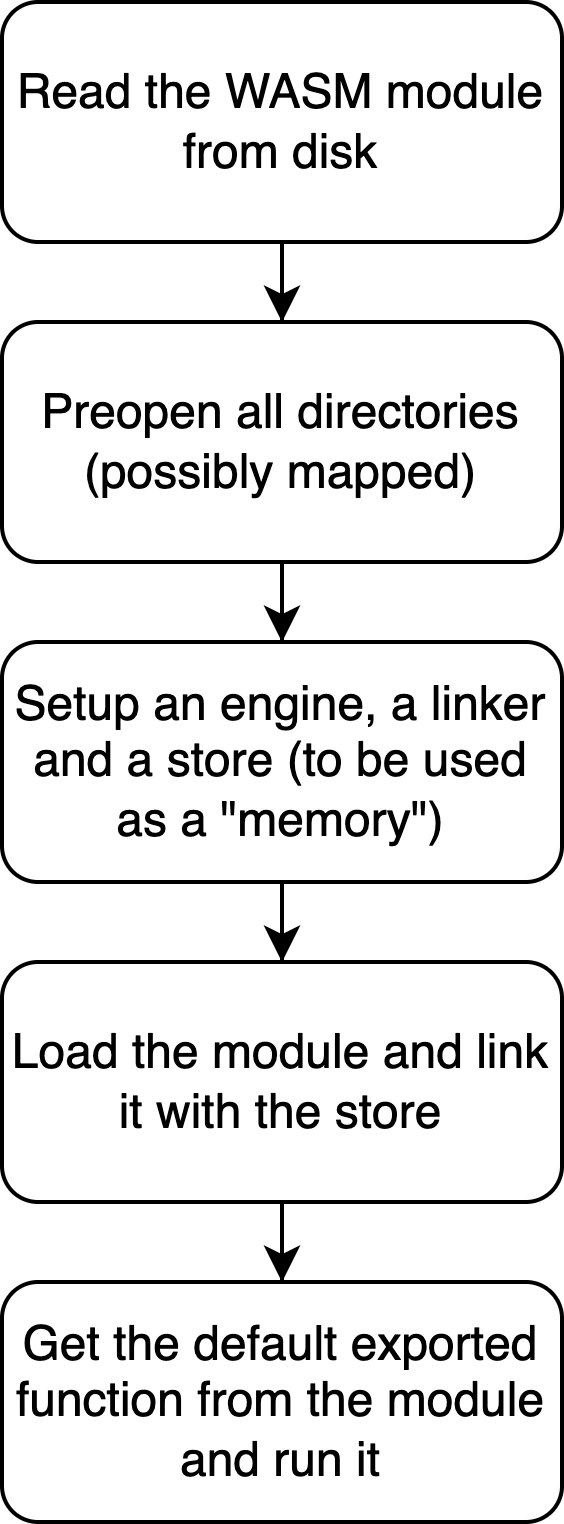
\includegraphics[width=0.25\linewidth]{rs-landlock-wasm.png}
  \caption{A high-view diagram of how the \texttt{wasm} module operates.}
  \label{fig:wasm-module}
\end{figure}

\subsubsection{The \texttt{landlock} module}

The \texttt{landlock} module is a thin wrapper around the API made available by the \textit{rust-landlock} crate.
It handles mostly ruleset creation, rule insertion, and enforces the policies before the desired WASM module is run.
The main outline of the code is visible in Listing \ref{lst:rust-landlock}.

\subsubsection{The \texttt{path\_access} module}

The \texttt{landlock} module makes use of another thin wrapper, the \texttt{PathAccess} struct defined
in the \texttt{path\_access} module.
Here, the main entity is the \texttt{PathAccess} struct, that tracks which flags, as defined in Table \ref{table:landlock-flags},
are applied to a single path. The flags list starts empty, and multiple flags can be added at any times.
Moreover, this module also takes care of conversions between types required by the Landlock ABI in order
to make the code compile.

\subsection{Available permission settings}

The program allows to specify all access right flags from the first version of the Landlock
ABI\footnote{At the moment it is not possible to specify the \texttt{LANDLOCK\_ACCESS\_FS\_REFERER} in order to reparent a file hierarchy.},
which are listed in Table \ref{table:landlock-flags}.

\vspace*{0.5cm}
\begin{code}[language=Rust, caption=The outline of the \texttt{landlock} module., label=lst:rust-landlock]
pub struct Landlock {
  ruleset: RulesetCreated,
}

impl Landlock {
  // Creates a new ruleset with flags from
  // Landlock ABI version 1
  pub fn new() -> Result<Self, RulesetError> {...}

  // Add a set of rules to the ruleset
  pub fn add_rules(
    mut self,
    rules: impl Iterator<Item = PathAccess>)
    -> Result<Self>
  {...}

  // Add a single rule to the ruleset
  pub fn add_rule(
    mut self,
    path_access: PathAccess) -> Result<Self>
  {...}

  // Self restrict the process and checks whether Landlock
  // is supported or not by the running kernel
  pub fn enforce(self) -> Result<RestrictionStatus>
  {...}
}
\end{code}

\clearpage\noindent
The following examples illustrate how to combine some of them:
\begin{itemize}
  \item \texttt{file:R} allows only to read from \textit{file};
  \item the combination of \texttt{file:X} and \texttt{.:RDir} allows the execution of \textit{file} and the listing of the current directory;
  \item \texttt{.:MReg} only allows the creation, rename or linking of regular files in the current directory;
  \item \texttt{.:R,W} and \texttt{./subdir:*} allows only reads and writes on files in the current directory, while no restrictions are
        made for \textit{subdir}.
\end{itemize}

Note that the directories containing the files of interest must always be preopened,
even if their content is then restricted by Landlock. This is because the preopen operation
is required by the WebAssembly runtimes, while specific permissions are handled by Landlock.

The Landlock self-restriction is applied after the necessary preopening of the directories,
otherwise the running process would have to always have the permissions for listing directories even if
not needed by the WASM binary.

\begin{table}[hbt]
  \centering
  \begin{tabular}{|l|l|}
    \hline
    \textit{Flag} & \textit{Enabled permission} \\ \hline\hline
    \texttt{X} & Execute a file \\ \hline
    \texttt{W} & Write to a file \\ \hline
    \texttt{R} & Read a file \\ \hline
    \texttt{RDir} & Open a directory or list its content \\ \hline
    \texttt{DDir} & Delete an empty directory or rename one \\ \hline
    \texttt{D} & Unlink or rename a file \\ \hline
    \texttt{MChar} & Create, rename or link a character device \\ \hline
    \texttt{MDir} & Create or rename a directory \\ \hline
    \texttt{MReg} & Create, rename or link a regular file \\ \hline
    \texttt{MSock} & Create, rename or link a socket \\ \hline
    \texttt{MFifo} & Create, rename or link a named pipe \\ \hline
    \texttt{MBlock} & Create, rename or link a block device \\ \hline
    \texttt{MSym} & Create, rename or link a symbolic link \\ \hline
    \texttt{$\sim$read} & Combination of \texttt{X}, \texttt{R} and \texttt{RDir} \\ \hline
    \texttt{$\sim$write} & Combination of all but \texttt{X}, \texttt{R} and \texttt{RDir} \\ \hline
    \texttt{*} & Enable all flags \\ \hline
  \end{tabular}
  \caption{Provided flags and corresponding Landlock permissions.}
  \label{table:landlock-flags}
\end{table}

\subsection{Advantages and disadvantages}

The main advantage that Landlock brings is simplicity. For the developer, the API is simple enough to use,
and it can be used in a variety of languages - the main three languages are C (used directly with the kernel libraries),
Rust (as in this project), and Go\footnote{\url{https://github.com/landlock-lsm/go-landlock}}.
From the user's point of view, the provided permission flags are clear enough that it is required to have
only a basic understanding of Linux's file system permissions.
Hence, it can be used to provide a clear interface that is not so different from the one already given by
the existing runtimes.
Moreover, Landlock allows \textit{unprivileged} access control - it is not necessary to gain particular privileges
when running a binary, so the user can run a WebAssembly module in a protected environment even if they are not
in the \textit{sudoers} group.

The biggest drawback with this approach is simplicity itself. As highlighted in Section \ref{sec:intro-lsm-landlock},
there is no way to define exceptions - this restricts the possibilities given to the user, and makes some situations
impossible to specify. For example, if a \texttt{LANDLOCK\_ACCESS\_FS\_REMOVE\_FILE} right is given to a directory,
all files in that directory can be renamed and there is no way to prevent renaming for a specific file.
Or similarly, if we have give the \texttt{LANDLOCK\_ACCESS\_FS\_READ\_FILE} and \texttt{LANDLOCK\_ACCESS\_FS\_WRITE\_FILE}
permissions on a certain directory, then all files that are children of that directory can be read or written, even
if they are inside subdirectories. If we then try to ``restrict'' this behaviour by giving only read permissions to
certain subdirectories, they would still have the write permissions from the parent directory.
In addition to this, the set of capabilities is somewhat limited, and mostly related to the file system.

\section{Restricting the WASI sandbox with eBPF}
\label{sec:restricting-wasi-ebpf}

\textit{BPFContain} \cite{bpfcontain} is a container security daemon for Linux written in Rust that offers
interoperability with \textit{eBPF} \cite{ebpf}.
Since \textit{BPFContain} is an external tool and not a library such as \textit{rust-landlock}, there was no need
to develop a project from scratch, since it is possible to combine it with the WebAssembly runtime of choice, which
in our case is \textit{Wasmtime}.

It should be noted that \textit{BPFContain} is still in active development and not yet feature-complete.
Finally, for this tool to work, BPF should be enabled when compiling the Linux kernel.

\subsection{Usage}

The usage is pretty straightforward:
\begin{enumerate}
  \item run the daemon once in the foreground in order to create the work files and directories -
        these are mostly log files and a directory used for the policies in \texttt{/var/lib/bpfcontain},
        which permissions are set so that its content is readable, writable and executable by the daemon;
  \item create a policy in \texttt{/var/lib/bpfcontain/policy};
  \item start the daemon with super user privileges;
  \item run confined program by referring the policy name, and the policy itself can be written in YAML.
\end{enumerate}

\subsection{Available permission settings}

The number of permission options that is possible to specify is way greater than the one offered by Landlock.
A policy is hence separated into multiple parts:
\begin{itemize}
  \item a \textit{name} for the policy file and a \textit{command} to run, both required;
  \item an optional set of \textit{rights} to grant; a right can appear in different forms, such as:
        \begin{itemize}
          \item a right on specific devices, such as \texttt{terminal} or \texttt{/dev/null};
          \item a grant on a particular folder or file, which is usually a combination of the classic \texttt{rwxa} permissions;
          \item access to the kernel's capabilities (e.g., DAC override);
          \item a list of process names with which communication is allowed;
          \item a list of primitives that the program can use on the network (such as client, send, recv).
        \end{itemize}
  \item an optional set of \textit{restrictions} to explicitly revoke, which follows the same structure as the
        granted rights;
  \item and finally an optional set of \textit{taint rules}, which again follow the same structure described above.
\end{itemize}

Specifically, when a policy is \textit{tainted}, BPFContain will start enforcing it. This means that a policy
can be loaded by BPFContain but not be enforced until the controlled program does a specific
action (e.g., access the network or send a message to a process).
This however must be explicitly declared in the policy, since all policies are tainted, hence enforced, by default.

An example of a policy is defined in Listing \ref{lst:yaml-policy-bash}, which defines how to
run \textit{bash} in a confined environment.
In this policy, \textit{bash} is allowed to access the terminal and \texttt{/dev/null}, as well
as reading and executing everything in \texttt{/} and reading everything in \texttt{/proc}.
An important point is the \texttt{deny} section - here \textit{bash} is prevented to writing and
appending anything in all of the file system.
Lastly, this policy is not active by default, but the process become ``tainted'' and the policy is enforced
when \textit{bash} tries to write or append anywhere in the file system.

A more complex example is shown in Listing \ref{lst:yaml-policy-httpd}, which shows a policy
used to run \textit{httpd}, allowing reading the files to serve, reading and appending to log files,
and allowing inter-process communication only with running \textit{mysqld} processes.

In the specific case of WebAssembly, it is enough to simply set the \texttt{cmd} option as
a call to the WASI runtime with the desired binary, \textit{Wasmtime} or \textit{Wasmer}, making sure that
necessary directories are preopened and eventual environment variables are imported.
An example policy is visible in Listing \ref{lst:yaml-policy-wasm}, where \textit{copy-file.wasm} simply copies
the content of \texttt{input.txt} to \texttt{output.txt}.

\vspace*{0.5cm}
\begin{code}[language=yaml, caption=A policy for running bash., label=lst:yaml-policy-bash]
# Name and command of the policy
name: bash
cmd: /bin/bash
defaultTaint: false

allow:
  # Allow access to terminal and /dev/null
  - device: terminal
  - device: null

  # Allow read and execute access on the file system
  - fs: {pathname: /, access: rxm}
  - fs: {pathname: /proc, access: r}

deny:
  # Prevent writes
  - fs: {path: /, access: wa}

taint:
  - fs: {path: /, access: wa}
\end{code}

\begin{code}[language=yaml, caption=Running WASM with BPFContain., label=lst:yaml-policy-wasm]
# Name and command of the policy
name: copy-file
cmd: wasmtime --dir=. copy-file.wasm

allow:
  - fs: {pathname: ., access: rwxm}
\end{code}

\begin{code}[language=yaml, caption=A policy for HTTPD., label=lst:yaml-policy-httpd]
# Name and command of the policy
name: httpd
cmd: httpd

allow:
  # Allow access to terminal and /dev/null
  - dev: random
  - dev: null

  # Access to log files
  - file: {pathname: /var/log/httpd, access: rw}
  - file: {pathname: /var/log/httpd/*.log, access: ra}

  # Read configuration
  - file: {pathname: /etc/httpd, access: r}

  # Serve files
  - file: {pathname: /srv, access: r}

  # Read hostname information
  - file: {pathname: /etc/host*, access: r}

  # Shared libraries loaded at runtime
  - file: {pathname: /usr/lib/httpd/modules/*.so,
           access: mr}
  - file: {pathname: /usr/lib/libnss*.so.*, access: mr}
  - file: {pathname: /usr/lib/libgcc_s.so.*, access: mr}

  # Allow ipc with MySQL
  - ipc: mysqld

  # Allow sending signals to existing httpd instances
  - signal: {to: httpd, signals: [check, superFatal]}

  # Use networking
  - net: [server, send, recv]
\end{code}

\subsection{Advantages and disadvantages}

The main advantage of using \textit{eBPF} is the extreme customisation in defining all the
permissions and capabilities that a process can have. Most notably, when comparing with Landlock,
there is support for exceptions and restrictions, so that more cases can be covered.

A point of note is the ability to restrict communication with other processes, be it by allowing
or disallowing IPC, or specifying what signals can be send and to whom.
Moreover, the restrictions and permissions applied to files and directories are more specific and do not
necessarily transfer to subdirectories. As seen in the example in the previous sections,
one can also use \textit{wildcards} when describing paths, such as the \texttt{/var/log/httpd/*log}
in Listing \ref{lst:yaml-policy-httpd}.

Finally, other desirable permissions are covered, such as network and devices. Network was also present
in Landlock, but only regarding the creation and management of sockets. Similarly, Landlock offered
creating, renaming and linking devices, but eBPF allows to specify which particular devices can be accessed
and which not.

However, eBPF brings also some disadvantages that Landlock does not have.
The biggest downside is regarding usability - while Landlock can be used by anyone able to use
the terminal and understand the basics of passing parameters, BPFContain requires the writing
of a policy in a specific language, albeit a simple one like YAML, and this policy must be in a very
specific location\footnote{To be fair, this is a limitation of \textit{BPFContain} and not of \textit{eBPF} itself.}.
This obviously decreases the level of simplicity and usability for a user that wants to contain and restrict
some binaries.

Another point regarding the specific usage with \textit{Wasmtime} and WebAssembly is the necessity of
having executable privileges - since \textit{Wasmtime} offers a command line binary, then in order to run
a WebAssembly module the confined process must be able to execute commands. This however transfers this
permission to the WebAssembly module itself. This permission can be restricted only to a specific file system
location, but it is still something that has to be taken into consideration.

Lastly, with this method it is necessary to run a \textit{separate} daemon that does the actual
confinement, and this daemon must be run as a super user.
Hence, a user that is not able to use the \texttt{sudo} command is not able to leverage eBPF
expressive power.
This is in stark contrast with Landlock, which sets out to offer \textit{unprivileged} access control,
so that super user privileges are not required to enforce the sandbox restriction.